\documentclass[11pt,a4paper]{article}

% ---------- Packages ----------
\usepackage[utf8]{inputenc}
\usepackage[T1]{fontenc}
\usepackage{lmodern}
\usepackage{amsmath,amssymb}
\usepackage{enumitem}
\usepackage{geometry}
\usepackage{fancyhdr}
\usepackage[most]{tcolorbox}   % enhanced, breakable
\usepackage{hyperref}
\usepackage{circuitikz}

% ---------- Geometry ----------
\geometry{margin=2.5cm}

% ---------- Header/Footer ----------
\setlength{\headheight}{14pt}  % fancyhdr warning verhindern
\pagestyle{fancy}
\fancyhf{}
\lhead{Einführung in die Elektrotechnik}
\rhead{Wintersemester 2025}
\cfoot{\thepage}

% ---------- Exercise Environment ----------
\newcounter{exercise}
\newenvironment{exercise}[1][]
  {\refstepcounter{exercise}%
   \begin{tcolorbox}[enhanced, breakable, width=\textwidth,
     colback=blue!5!white,colframe=blue!60!black,
     fonttitle=\bfseries\large,
     title=Aufgabe~\theexercise:~#1]}
  {\end{tcolorbox}}

% ---------- Solution Environment ----------
\newif\ifshowsolutions
\showsolutionstrue  % comment to hide solutions

\newenvironment{solution}
  {\ifshowsolutions
     \begin{tcolorbox}[enhanced, breakable, width=\textwidth,
       colback=green!5!white,colframe=green!50!black,
       fonttitle=\bfseries\large,
       title=Lösung]}
  {\end{tcolorbox}\fi}

% ---------- Document ----------
\begin{document}

% ----- Header Box -----
\begin{tcolorbox}[enhanced, breakable, colback=gray!10!white,
  colframe=gray!70!black, fonttitle=\bfseries\large,
  title={Aufgabenblatt \#3}: DC 2: Netzwerkanalyse und Leistung, sharp corners, width=\textwidth]
\begin{center}
  Besprechung: 29.10.2025
\end{center}
\end{tcolorbox}
\vspace{1cm}

% ----- Exercise 1 -----
\begin{exercise}[Systematische Netzwerkanalyse]
Das folgende Netzwerk enthält die Widerstände $R_1 = 1\,\Omega$, $R_2 = 2\,\Omega$, $R_3 = 5\,\Omega$, $R_4 = 25\,\Omega$ und $R_5 = 40\,\Omega$ sowie die Quellspannungen $U_{q1} = 16.2\,\mathrm{V}$ und $U_{q2} = 11.4\,\mathrm{V}$. Es sind alle Zweigströme zu bestimmen.

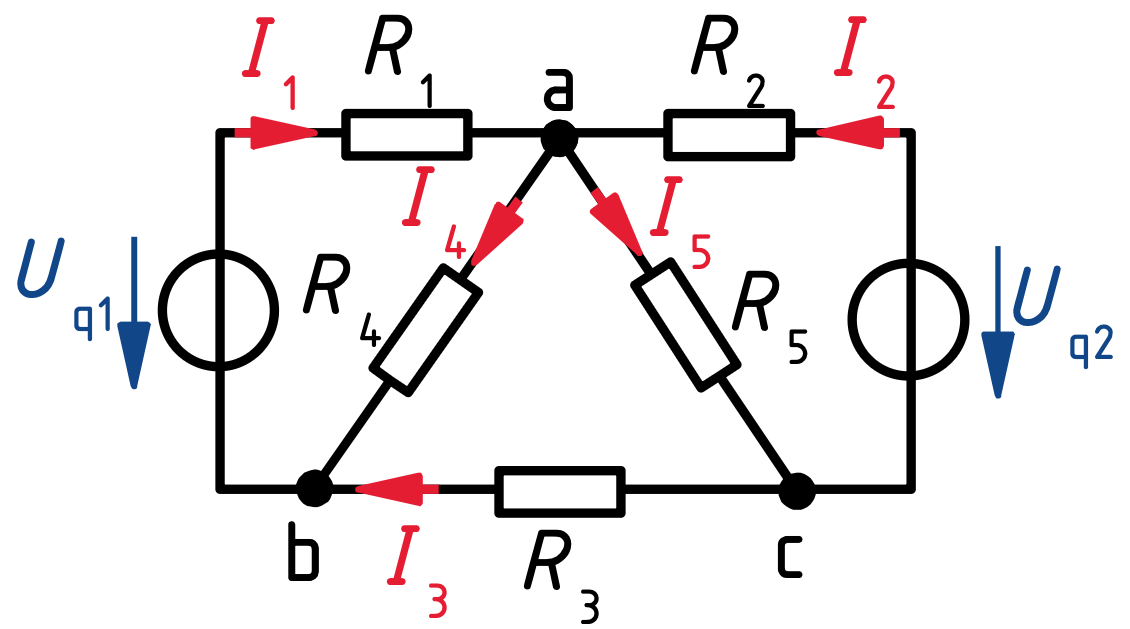
\includegraphics[width=0.7\textwidth]{figures/complete_tree_1.png}
\end{exercise}

\ifshowsolutions
\begin{solution}
Das Netzwerk hat $n = 3$ Knoten, also gibt es $n - 1 = 2$ linear unabhängige Knoten-Gleichungen. Wir wählen die Knoten $B$ und $C$:
\[
I_3 + I_4 - I_1 = 0
\]
\[
I_5 - I_2 - I_3 = 0
\]

Die Anzahl der Zweige ist 5, also gibt es $5 - (3 - 1) = 3$ linear unabhängige Maschengleichungen. Darstellung des Netzwerks mit einem ausgewählten vollständigen Baum (rot markiert):

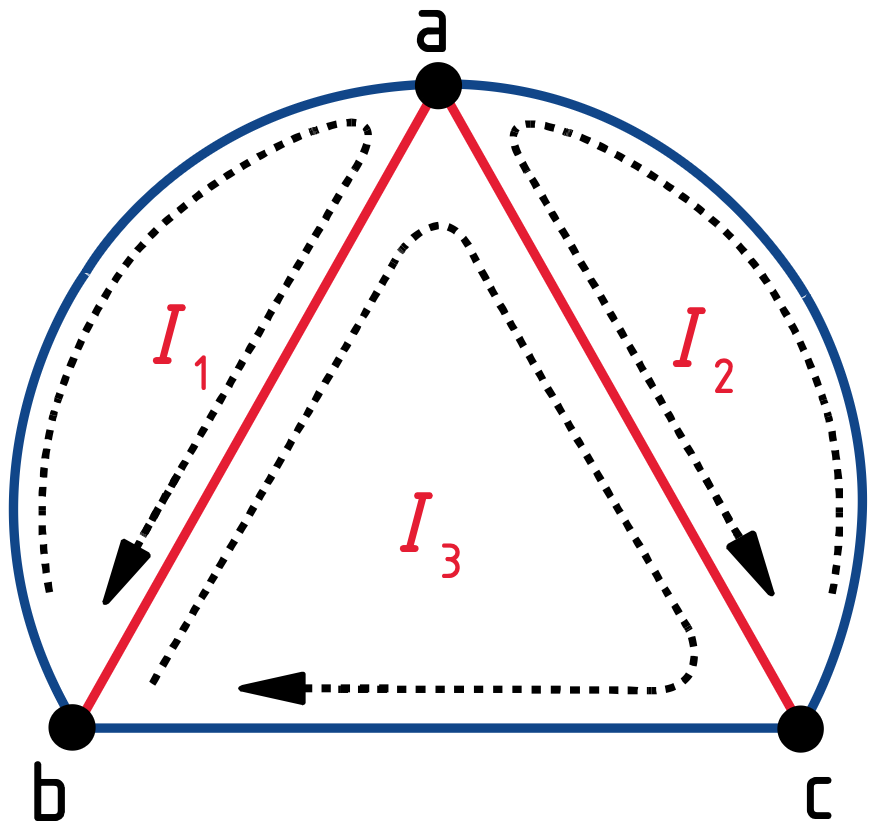
\includegraphics[width=0.4\textwidth]{figures/complete_tree_2.png}

Die Zweigströme in den Verbindungszweigen, also $I_1$, $I_2$ und $I_3$, werden als Maschenströme gewählt. Die Maschengleichungen werden durch Durchlaufen der Maschen in Richtung der Zählpfeile der Maschenströme aufgestellt:
\[
\begin{aligned}
M_1 &: \quad R_1 I_1 + R_4 I_4 - U_{q1} = 0 \\
M_2 &: \quad R_2 I_2 + R_5 I_5 - U_{q2} = 0 \\
M_3 &: \quad R_3 I_3 - R_4 I_4 + R_5 I_5 = 0
\end{aligned}
\]

Resultierendes Gleichungssystem in Matrixform:
\[
\begin{bmatrix}
-1 & 0 & 1 & 1 & 0 \\
0 & -1 & -1 & 0 & 1 \\
R_1 & 0 & 0 & R_4 & 0 \\
0 & R_2 & 0 & 0 & R_5 \\
0 & 0 & R_3 & -R_4 & R_5
\end{bmatrix}
\begin{bmatrix}
I_1 \\[4pt] I_2 \\[4pt] I_3 \\[4pt] I_4 \\[4pt] I_5
\end{bmatrix}
=
\begin{bmatrix}
0 \\[4pt] 0 \\[4pt] U_{q1} \\[4pt] U_{q2} \\[4pt] 0
\end{bmatrix}.
\]
Einsetzen der numerischen Werte ergibt:
\[
\begin{bmatrix}
-1 & 0 & 1 & 1 & 0 \\
0 & -1 & -1 & 0 & 1 \\
1 & 0 & 0 & 25 & 0 \\
0 & 2 & 0 & 0 & 40 \\
0 & 0 & 5 & -25 & 40
\end{bmatrix}
\begin{bmatrix}
I_1 \\[4pt] I_2 \\[4pt] I_3 \\[4pt] I_4 \\[4pt] I_5
\end{bmatrix}
=
\begin{bmatrix}
0 \\[4pt] 0 \\[4pt] 16.2 \\[4pt] 11.4 \\[4pt] 0
\end{bmatrix}.
\]
...
\[
I_1 = 1.2\,\mathrm{A}, \qquad
I_2 = -0.3\,\mathrm{A}, \qquad
I_3 = 0.6\,\mathrm{A}, \qquad
I_4 = 0.6\,\mathrm{A}, \qquad
I_5 = 0.3\,\mathrm{A}.
\]
\end{solution}
\fi

% ----- Exercise 2 -----
\begin{exercise}[Thévenin und Leistungsanpassung]
Der variable Widerstand $R$ wird so eingestellt, dass er die maximale Leistung aus der Schaltung aufnimmt.
\begin{enumerate}[label=\alph*)]
    \item Berechne den Wert von $R$ für maximale Leistung.
    \item Bestimme die maximal von $R$ aufgenommene Leistung.
\end{enumerate}

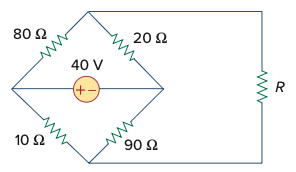
\includegraphics[width=0.7\textwidth]{figures/maximum_power.png}
\end{exercise}

\ifshowsolutions
\begin{solution}
\begin{enumerate}[label=\alph*)]
\item Zunächst berechnen wir den Thévenin-Äquivalenzwert, von den Klemmen von R aus betrachtet.

Hierfür sei das Potential am Knoten $D$ (links der $40\, \mathrm{V}$-Quelle) $40\, \mathrm{V}$ und am Knoten $B$ (rechts der Quelle) $0\, \mathrm{V}$.

Für den oberen Knoten $A$:
\[
\frac{V_A - 40}{80} + \frac{V_A - 0}{20} = 0
\Rightarrow 5V_A - 200 = 0
\Rightarrow V_A = 8\, \mathrm{V}
\]

Für den unteren Knoten $C$:
\[
\frac{V_C - 40}{10} + \frac{V_C - 0}{90} = 0
\Rightarrow 9V_C - 360 = 0
\Rightarrow V_C = 36\, \mathrm{V}
\]

Demnach ist die Leerlaufspannung (Thévenin-Spannung):
\[
V_\mathrm{th} = |V_A - V_C| = |8 - 36| = 28\, \mathrm{V}
\]

Nun deaktivieren wir die $40\, \mathrm{V}$-Quelle (ersetzen durch einen Kurzschluss):
\[
R_A = (80\, \Omega \parallel 20\, \Omega) = \frac{80 \cdot 20}{80 + 20} = 16\, \Omega
\]
\[
R_C = (10\, \Omega \parallel 90\, \Omega) = \frac{10 \cdot 90}{10 + 90} = 9\, \Omega
\]

Da $R_A$ und $R_C$ in Reihe geschaltet sind,
\[
R_\mathrm{th} = R_A + R_C = 16 + 9 = 25\, \Omega.
\]

Für maximale Leistung: $R = R_\mathrm{th} = 25\, \Omega$

\item Die Schaltung kann durch eine Thévenin-Spannungsquelle $V_\mathrm{th}$ in Serie mit einem Thévenin-Widerstand $R_\mathrm{th}$ und einer Last $R_L$ dargestellt werden.
\[
I = \frac{V_{\text{th}}}{R_{\text{th}} + R_L}
\]

Leistung im Lastwiderstand:
\[
P = I^2 R_L = \frac{V_\mathrm{th}^2 R_L}{(R_\mathrm{th} + R_L)^2}
\]

Einsetzen von $R_L = R_\mathrm{th}$ in die Leistungsformel:
\[
P_{\max} = \frac{V_\mathrm{th}^2 R_\mathrm{th}}{(R_\mathrm{th} + R_\mathrm{th})^2} = \frac{V_\mathrm{th}^2}{4 R_\mathrm{th}} = \frac{28^2}{4 \cdot 25} = \frac{784}{100} = 7.84\, \mathrm{W}
\]
\end{enumerate}
\end{solution}
\fi

% ----- Exercise 3 -----
\begin{exercise}[Effizienz]
Bestimme die jeweiligen Bruchteile der maximalen Lastleistung bei folgenden Effizienzen.
\begin{enumerate}[label=\alph*)]
    \item $\eta = 75\%$
    \item $\eta = 90\%$
\end{enumerate}
\end{exercise}

\ifshowsolutions
\begin{solution}
Die Effizienz $\eta$ ist definiert als das Verhältnis der an die Last abgegebenen zur insgesamt von der Quelle gelieferten Leistung.

Für eine Thévenin-Quelle ($V_\mathrm{th}$, $R_\mathrm{th}$) mit einer Last $R_L$ ist die Effizienz:
\[
\eta = \frac{P_L}{P_L + P_\mathrm{th}} = \frac{R_L}{R_L + R_\mathrm{th}}
\]

Bei maximaler Leistung ($R_L = R_\mathrm{th}$): 
\[
P_{L,\max} = \frac{V_\mathrm{th}^2}{4 R_\mathrm{th}}
\]

Demnach ist das Leistungs-Verhältnis:
\[
\frac{P_L}{P_{L,\max}} = \frac{ \dfrac{V_\mathrm{th}^2 R_L}{(R_\mathrm{th} + R_L)^2} }{ \dfrac{V_\mathrm{th}^2}{4 R_\mathrm{th}} } = 4 R_\mathrm{th} \cdot \frac{R_L}{(R_\mathrm{th} + R_L)^2}
\]

\begin{enumerate}[label=\alph*)]
\item Für $\eta = 75\%$:
\[
0.75 = \frac{R_L}{R_L + R_\mathrm{th}}
\]
\[
\Rightarrow R_L = 3 R_\mathrm{th}
\]
\[
\Rightarrow \frac{P_L}{P_{L,\max}} = 4R_\mathrm{th} \cdot \frac{3R_\mathrm{th}}{(R_\mathrm{th} + 3R_\mathrm{th})^2} = \frac{12R_\mathrm{th}^2}{(4R_\mathrm{th})^2} = 0.75
\]
Sogar wenn die Effizienz auf 75\% steigt, erhält die Last immer noch 75\% der maximal möglichen Leistung. Somit wird eine deutlich höhere Effizienz auf Kosten einer nur moderaten Reduktion der an die Last abgegebenen Leistung erreicht.
\item Für $\eta = 90\%$:
\[
0.9 = \frac{R_L}{R_L + R_\mathrm{th}}
\]
\[
\Rightarrow R_L = 9 R_\mathrm{th}
\]
\[
\Rightarrow \frac{P_L}{P_{L,\max}} = 4 R_\mathrm{th} \cdot \frac{9 R_\mathrm{th}}{(R_\mathrm{th} + 9 R_\mathrm{th})^2} = \frac{36 R_\mathrm{th}^2}{(10 R_\mathrm{th})^2} = 0.36
\]
Für sehr hohe Effizienzen fällt die an die Last abgegebene Leistung also deutlich ab.
\end{enumerate}
\end{solution}
\fi

% ----- Exercise 4 -----
\begin{exercise}[Leistungsmessung]
Berechne den Einfluss der Platzierung von Voltmeter und Amperemeter auf die gemessene Leistung in einer Gleichstrom-Widerstandsschaltung mit den unten angegebenen Parametern und Konfigurationen. Vergleiche die gemessene Leistung mit der tatsächlich im Lastwiderstand umgesetzten Leistung für beide Konfigurationen und für die beiden unterschiedlichen Lastwiderstände.

\begin{itemize}
  \item Quellspannung: $V_s = 12\, \mathrm{V}$
  \item Innenwiderstand der Quelle: $R_s = 1\, \Omega$
  \item Innenwiderstand des Voltmeters: $R_v = 1000\, \Omega$
  \item Innenwiderstand des Amperemeters: $R_a = 0.1\, \Omega$
  \item Lastwiderstand (zwei Fälle):
  \begin{itemize}
      \item Niedriger Lastwiderstand: $R_L =  1\, \Omega$
      \item Hoher Lastwiderstand: $R_L = 100\, \Omega$
  \end{itemize}
\end{itemize}

\begin{enumerate}
  \item Konfiguration A (Strom-richtig):\\
  Voltmeter über der Quelle, Amperemeter in Reihe mit der Last.\\

\begin{center}
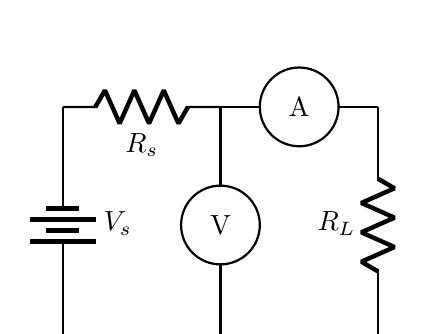
\begin{tikzpicture}[thick, scale=1.0]
  % Source with internal resistance
  \draw (0,0) to[battery, l_={$V_s$}] (0,3);
  \draw (0,3) to[resistor, l_={$R_s$}] (2,3);

  % Ammeter (as a circle)
  \draw (2,3) -- (2.5,3);
  \draw (3,3) node[circle,draw,minimum size=10mm,inner sep=0pt]{A};
  \draw (3.5,3) -- (4,3);

  % Load resistor
  \draw (4,3) to[resistor, l_={$R_L$}] (4,0);

  % Return path
  \draw (4,0) -- (0,0);

  % Voltmeter (as a circle)
  \draw (2,1.5) node[circle,draw,minimum size=10mm,inner sep=0pt]{V};
  \draw (2,0) -- (2,1);
  \draw (2,2) -- (2,3);
\end{tikzpicture}
\end{center}

  \item Konfiguration B (Spannungs-richtig):\\
  Voltmeter über der Last, Amperemeter in Reihe mit der Quelle.\\
\end{enumerate}
\end{exercise}

\ifshowsolutions
\begin{solution}
\paragraph{Konfiguration A}
\[
I_s = I_L + I_v
\]
\[
I_L=\frac{V_t}{R_a + R_L}\quad\text{(durch Amperemeter und Last)}
\]
\[
I_v=\frac{V_t}{R_v}\quad\text{(durch Voltmeter)}.
\]

Quellklemmen:
\[
V_t = V_s - R_s \cdot I_s = \frac{V_s}{1 + R_s \left(\frac{1}{R_a + R_L} + \frac{1}{R_v}\right)}
\]

Gemessene Leistung (was man aus den Messwerten der Messgeräte berechnen würde, d.h. Voltmeter~$\times$~Amperemeter):
\[
P_{\text{meas},A} = V_t I_L = \frac{V_t^2}{R_a + R_L} = \frac{V_s^2}{(R_a + R_L) (1 + R_s \left(\frac{1}{R_a + R_L} + \frac{1}{R_v}\right)^2}
\]

Tatsächlich im Lastwiderstand umgesetzte Leistung:
\[
P_\text{true}=I_L^2 R_L = \dfrac{V_t^2\,R_L}{(R_a + R_L)^2}
\]

\paragraph{Konfiguration B}
\[
R_p = \frac{R_L R_v}{R_L + R_v} \quad\text{(Parallelschaltung von Last und Voltmeter)}
\]
\[
I_s = \frac{V_s}{R_s + R_a + R_p}
\]
\[
V_L = I_s \, R_p \quad\text{(Spannung an Last und Voltmeter)}
\]

Gemessene Leistung:
\[
P_{\text{meas},B} = V_L I_s = I_s^2 R_p = \frac{V_s^2 R_p}{(R_s + R_a + R_p)^2}
\]

Tatsächlich im Lastwiderstand umgesetzte Leistung:
\[
P_\text{true} = I_L^2 R_L
\]
\[
I_L = \frac{V_L}{R_L} = \frac{I_s R_p}{R_L}
\]
\[
\Rightarrow P_\text{true} = \frac{I_s^2 R_p^2}{R_L}
\]

\begin{center}
\begin{tabular}{lrrrrr}
\hline
$R_L$ & $P_\text{true}$ & $P_{\text{meas},A}$ & $P_{\text{meas},B}$ \\
\hline
$1\, \Omega$ & $32.62\, \mathrm{W}$ & $35.88\, \mathrm{W}$ & $32.65\, \mathrm{W}$ \\
$100\, \Omega$ & $1.406\, \mathrm{W}$ & $1.407\, \mathrm{W}$ & $1.546\, \mathrm{W}$ \\
\hline
\end{tabular}
\end{center}
\end{solution}
\fi

\end{document}